\documentclass[12pt, a4paper]{article}
\usepackage[UTF8]{ctex}
\usepackage{amsmath}
\usepackage{amssymb}
\usepackage{amsthm}
\usepackage{geometry}
\usepackage{enumitem}
\usepackage{indentfirst}
\usepackage{caption}
\usepackage{fancyhdr}
\usepackage{booktabs}
\usepackage{titlesec}
\usepackage{draftwatermark}%水印
\usepackage{graphicx} % 导入图像的宏包、单图
% 页面布局设置
\geometry{top=2.54cm, bottom=2.54cm, left=3.18cm, right=3.18cm}

\SetWatermarkText{B站：布加拉提}
\SetWatermarkScale{0.4}

% 行距设置
\linespread{1.5}

% 段落设置
\setlength{\parindent}{2em}
\setlength{\parskip}{0.5em}

% 节标题格式设置
\titleformat{\section}{\normalfont\Large\bfseries}{第\chinese{section}章、}{1em}{}
\titlespacing{\section}{0pt}{2.5ex plus 1ex minus .2ex}{1.3ex plus .2ex}

% 定理环境设置
\newtheoremstyle{solution}
{}
{}
{}
{}
{\bfseries}
{、}
{1em}
{}
\theoremstyle{solution}
\newtheorem{sol}{解}

% 页眉页脚设置
\pagestyle{fancy}
\fancyhf{}
\fancyhead[C]{b站布加拉提整理（回忆版）b站甘茶w独家讲解}
\fancyfoot[C]{\thepage}

\rfoot{整理人：八方\\资源提供：考研乔瑟夫}
\lhead{
\includegraphics[width=0.06\linewidth]{p1.png}}
\rhead{
\includegraphics[width=0.06\linewidth]{p2.png}}
\renewcommand{\headrulewidth}{0.4pt}
\renewcommand{\footrulewidth}{0.4pt}

\begin{document}

\begin{center}
\Large\textbf{2016哈工大硕士考试试题：805物理光学}
\end{center}





\section*{一、填空题（20分）}
\begin{enumerate}
    \item 一束光从空气以55度入射角进入到各向同性的透明介质中，此时光能量没有损失，这种介质的折射率为\_\_\_\_\_，入射光的偏振态为\_\_\_\_\_。
    \item 光波波函数中复振幅的物理含义是\_\_\_\_\_。
    \item 平面电磁波在传播过程中，电场强度和磁场强度的关系是\_\_\_\_\_，电场强度和磁感应强度的关系是\_\_\_\_\_。
    \item 光波从一种介质通过界面进入另一种介质中，磁感强度\_\_\_\_\_连续，电场强度的\_\_\_\_\_连续。
    \item 用迈克尔逊干涉仪测微小位移，若入射波长为$628.9nm$，当移动反射镜时，干涉条纹移动了2048条，则反射镜移动了\_\_\_\_\_。
    \item 一束单色光的振幅为$E$，与其振动方向垂直的另一束单色光的振幅为$0.5E$，这两束光相遇区域的光强为\_\_\_\_\_。
    \item 再利用光脉冲进行光速测量的实验中，测量到的光脉冲的传播速度时\_\_\_\_\_速度。
    \item 菲涅尔方程给出了单色平面波在晶体中传播时，光波\_\_\_\_\_之间所满足的关系。
    \item 两个频率相同，振动方向相同而传播方向相反的单色光波叠加产生\_\_\_\_\_。相邻两个波节之间的距离为\_\_\_\_\_。
\end{enumerate}
\section*{二、选择题（21分）}
\begin{enumerate}
    \item 在白炽光入射的牛顿环中，同级圆环中相应于颜色蓝到红的空间位置是\_\_\_\_\_。 \\
    A.由内到外\quad B.由外到内\quad C.不变\quad D.随机变化
    \item 在直径较小圆屏菲涅尔衍射的几何阴影中心处\_\_\_\_\_。\\
    A.永远是个暗点 \quad B.永远是个亮点,强度只与入射光强有关 \quad C.有时是亮点有时是暗点 \quad D.永远是个亮点，强度随屏大小而变
    \item 下列什么现象说明光是横波\_\_\_\_\_。\\
    A.光的色散\quad B.光的衍射\quad C.光的干涉\quad D.光的偏振
    \item 在晶体中双折射的光束为\_\_\_\_\_。\\
    A.只可以一束寻常光和一束非常光\quad B.可以两束寻常光\quad C.可以两束非常光\quad D.不可以两束非常光
    \item 在杨氏双缝干涉中，相邻亮条纹或暗条纹的间隔与下列哪一种因素无关\_\_\_\_\_。\\
    A.干涉级次\quad B.双缝间距\quad C.屏到双缝的距离\quad D.光波的波长
    \item （重复）在真空中波长为\(\lambda\) 的单色光，再折射率为$n$ 的透明介质中从A传播到B，若A,B两点的相位差为3\(\pi\) ,则此路径AB地光程差为\_\_\_\_\_.\\(A)$1.5\lambda$ \qquad(B)$1.5n\lambda$ \qquad(C)$3\lambda$ \qquad(D)$1.5\lambda/n$
    \item 光强为$I_0$的自然光入射到透光轴方向相交60度的两块理想偏振片后，最后通过第二块偏振片的透射光强度与入射光强度$I_0$之比是\_\_\_\_\_。\\
    A.1/2 \quad B.1/4\quad C.1/8\quad D.1/16
\end{enumerate}
\section*{三、名词解释（18分）}
\begin{enumerate}
    \item 古恩-哈恩斯位移
    \item 群速度
    \item 电光效应
    \item 艾里斑
    \item 瑞利判据
    \item 双折射
\end{enumerate}
\section*{四、简答与画图题（30分）}
\begin{enumerate}
    \item 条纹对比度是表征光场相干程度的参量，影响条纹可见度的主要因素有哪些，简述空间相干性和时间相干性与个因素的关系
    \item 光波在金属表面反射与在玻璃表面反射相比，其反射光有什么特点？
    \item 什么是旋光1效应？法拉第磁光效应和自然旋光现象有何不同？
    \item 简述瑞利散射的主要特点。
    \item 简述折射率椭球的重要性质。
    \item 试在$yoz$平面画简图说明晶体中，光线面与法线面的关系。
\end{enumerate}
\section*{五、计算与分析（40分）}
\begin{enumerate}
    \item 太阳对地球的张角约为$32'$，太阳光的平均波长为$550nm$，若采用太阳光为光源，试计算杨氏干涉中两小孔的间距在多长范围内可观测到条纹，结果有何意义？
    \item 在下图所示干涉装置中，如果入射光的波长宽度为$0.05nm$，平均波长为$500nm$，问在小孔$S_1$处贴上多厚的玻璃片可以使$P$，点附近的条纹消失？玻璃片折射率为1.5
          \begin{figure}[!htb]
                \centering
                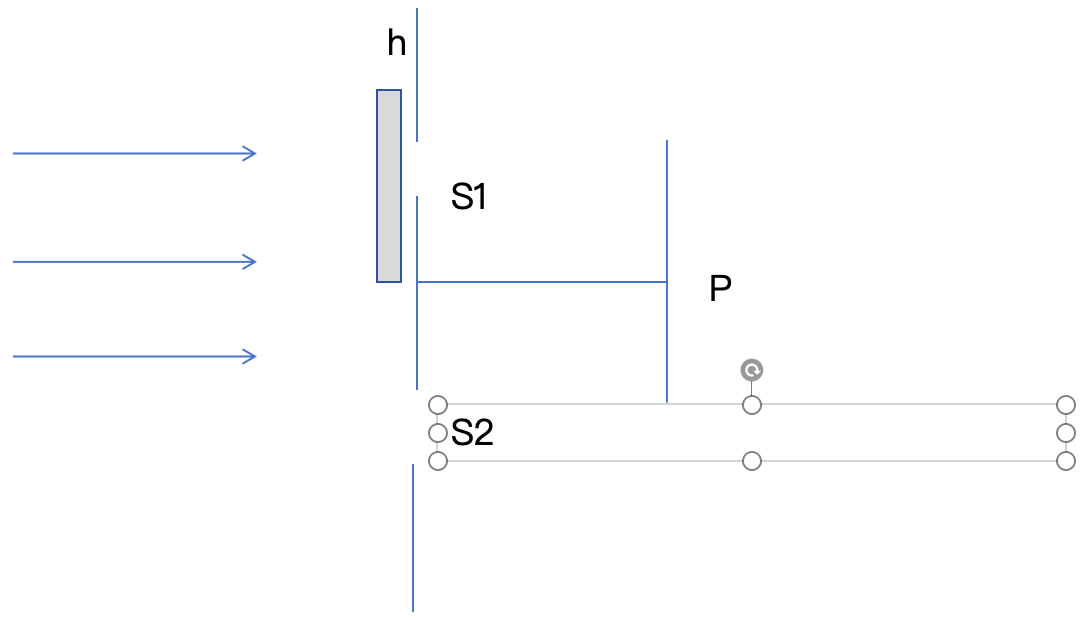
\includegraphics[width=0.4\linewidth]{161.png}              
          \end{figure}
    \item （重复） 以纳光观察迈克尔逊干涉条纹$\lambda=589.3nm$，先看到干涉场中12个亮环，且中心是亮点，然后移动一侧反射镜，看到中心消失了10个亮环，此时干涉场中还存在5个亮环。求：
          \begin{enumerate}
            \item 镜面移动的距离
            \item 开始时中心亮斑的级次
            \item 反射镜移动后，视场中最外那个亮环的干涉级
          \end{enumerate}
    \item 利用波长$\lambda=532.8nm$的激光测得某细丝的弗朗合费零级衍射条纹宽度为$1cm$，若透镜焦距为$40cm$，求该细丝直径。
    \item 使自然光相继通过三个偏振片，第一个与第三个偏振片的透光轴（从偏振片透出的偏振光的振动方向）正交，第二个偏振片的透光轴与第一片透光轴成45度角。若入射自然光的强度为$I_0$，问最后透出的光强是多少？
\end{enumerate}
\section*{六、论述题（15分）}
\begin{enumerate}
    \item 光学车间刚加工出三个性能良好的45度直角棱镜，表面未镀膜，他们折射率分别是1.35，1.60和1.91，试用一个小型准直光源和一个高精度照度计将他们区分出来，画出实验光路，并给出判断依据。
\end{enumerate}
\end{document}